    %% This is file `elsarticle-template-1-num.tex',
%%
%% Copyright 2009 Elsevier Ltd
%%
%% This file is part of the 'Elsarticle Bundle'.
%% ---------------------------------------------
%%
%% It may be distributed under the conditions of the LaTeX Project Public
%% License, either version 1.2 of this license or (at your option) any
%% later version.  The latest version of this license is in
%%    http://www.latex-project.org/lppl.txt
%% and version 1.2 or later is part of all distributions of LaTeX
%% version 1999/12/01 or later.
%%
%% The list of all files belonging to the 'Elsarticle Bundle' is
%% given in the file `manifest.txt'.
%%
%% Template article for Elsevier's document class `elsarticle'
%% with numbered style bibliographic references
%%
%% $Id: elsarticle-template-1-num.tex 149 2009-10-08 05:01:15Z rishi $
%% $URL: http://lenova.river-valley.com/svn/elsbst/trunk/elsarticle-template-1-num.tex $
%%
% \documentclass[preprint,12pt]{elsarticle}

%% Use the option review to obtain double line spacing
%% \documentclass[preprint,review,12pt]{elsarticle}

%% Use the options 1p,twocolumn; 3p; 3p,twocolumn; 5p; or 5p,twocolumn
%% for a journal layout:
% \documentclass[final,1p,times]{elsarticle}
\documentclass[final,1p,times,twocolumn]{elsarticle}
%% \documentclass[final,3p,times]{elsarticle}
%% \documentclass[final,3p,times,twocolumn]{elsarticle}
%% \documentclass[final,5p,times]{elsarticle}
%% \documentclass[final,5p,times,twocolumn]{elsarticle}

%% if you use PostScript figures in your article
%% use the graphics package for simple commands
%% \usepackage{graphics}
%% or use the graphicx package for more complicated commands
%% \usepackage{graphicx}
%% or use the epsfig package if you prefer to use the old commands
%% \usepackage{epsfig}

%% The amssymb package provides various useful mathematical symbols
\usepackage{amssymb}
\usepackage{lipsum}
%% The amsthm package provides extended theorem environments
%% \usepackage{amsthm}

%% The lineno packages adds line numbers. Start line numbering with
%% \begin{linenumbers}, end it with \end{linenumbers}. Or switch it on
%% for the whole article with \linenumbers after \end{frontmatter}.
% \usepackage{lineno}

%% natbib.sty is loaded by default. However, natbib options can be
%% provided with \biboptions{...} command. Following options are
%% valid:

%%   round  -  round parentheses are used (default)
%%   square -  square brackets are used   [option]
%%   curly  -  curly braces are used      {option}
%%   angle  -  angle brackets are used    <option>
%%   semicolon  -  multiple citations separated by semi-colon
%%   colon  - same as semicolon, an earlier confusion
%%   comma  -  separated by comma
%%   numbers-  selects numerical citations
%%   super  -  numerical citations as superscripts
%%   sort   -  sorts multiple citations according to order in ref. list
%%   sort&compress   -  like sort, but also compresses numerical citations
%%   compress - compresses without sorting
%%
%% \biboptions{comma,round}

% \biboptions{}

\usepackage{amsmath}% http://ctan.org/pkg/amsmath
\newcommand\sufr[3][0pt]{$\rule{0pt}{\dimexpr#1+1.4ex\relax}^\frac{#2}{#3}$}


\usepackage{graphicx}

\usepackage{algorithmic}
\usepackage{algorithm}

\usepackage{subfigure}
\usepackage{stfloats}

% \makeatletter
% \patchcmd{\@verbatim}
% {\verbatim@font}
% {\verbatim@font\small}
% {}{}
% \makeatother

\journal{Lancet Digital Health}

\begin{document}

\begin{frontmatter}

%% Title, authors and addresses

%% use the tnoteref command within \title for footnotes;
%% use the tnotetext command for the associated footnote;
%% use the fnref command within \author or \address for footnotes;
%% use the fntext command for the associated footnote;
%% use the corref command within \author for corresponding author footnotes;
%% use the cortext command for the associated footnote;
%% use the ead command for the email address,
%% and the form \ead[url] for the home page:
%%
%% \title{Title\tnoteref{label1}}
%% \tnotetext[label1]{}
%% \author{Name\corref{cor1}\fnref{label2}}
%% \ead{email address}
%% \ead[url]{home page}
%% \fntext[label2]{}
%% \cortext[cor1]{}
%% \address{Address\fnref{label3}}
%% \fntext[label3]{}

\title{DigiOnco: A Pipeline to Unveil Digital Non-Invasive Biomarkers from Multi-parametric Radiomics Footprints for the Indian Breast Cancer Cohort with Multiple Molecular Subtypes}

%% use optional labels to link authors explicitly to addresses:
% \author[label1,label2]{<author name>}
%  \address[label1]{<address>}
%  \address[label2]{<address>}

\author[label1]{Santhi Natarajan, Anand Ravishankar, Bharathi Malakreddy A }
\author[label2]{G.Lohith, Kritika Sekar, Shivakumar Swamy, Kumar Kallur, Basavalinga Ajai Kumar, Mahesh Bandimegal, Krithika Murugan}
\address[label1]{RadioGenomics Research Group, BMS Institute of Technology and Management, Visweswaraiah Technological Univesity, Bangalore, India}
\address[label2]{Health Care Global (HCG) Hospitals, Bangalore, India}

\begin{abstract}
%% Text of abstract
\textbf{Background}: Digital Imaging and Analytical Models (DIAMs) assisted Radiomics has emerged as a promising tool towards offering personalized therapeutics to patients. Oncological researchers seem to have benefited the most from the automated and reproducible analytics that DIAMs offer. However, statistical deductions and associations of inferences from DIAMs have to be cross-validated with a higher rate of concordance and robustness. With the amount of digital healthcare data amounting to 2.5 Zetabytes as on date, there is a dire need for standardization of DIAMs applied to cohort based study with heterogeneous patient centric parameters, including age, phenotypes and genotypes. 

\textbf{Methods}: DigiOnco, is a novel pipeline, intricately woven with carefully chosen set of Machine Learning (ML) algorithms. DigiOnco unveils the digital non-invasive biomarkers from multi-parametric Radiomics footprints obtained from the PET-CT imaging techniques. The hypothesis generation and validation is performed as both internal cross-validation as well as a retrospectively validated study. An independent cohort, having a set of external group of patients identified with breast cancer across multiple molecular subtypes, is used for the study.

\textbf{Findings}: The DigiOnco pipeline consists of multi-disciplinary stages involving both Radiomics and modern statistics. While Radiomics provides a real-world application based approach, statistical tools help to narrow down our biomarker search process. DigiOnco offers accuracy levels ranging from 72.7\% to 93.25\%, in mapping the feature sets to the various molecular subtypes of breast carcinoma. The internal cross validation and the retrospectively validated study on the cohort affirm our hypothesis. 

\textbf{Interpretation}: Considering the integration of our current findings with follow-up studies branching into other medical sub-doamins, the potential of homogenizing Machine Learning is huge in this field. The aim of obtaining the subset of optimal features from the radiomics feature set extracted from imaging, is to preserve the features with the highest level of information embedded in them. However it must also be duly noted that this pipeline is quite delicate when it comes to producing results, as the errors encountered in each step are rippled onto the subsequent stages. This is mitigated by having an optimal p-value level for the corresponding feature set. Furthermore, an increased sample size could help further fine tune the model. Additional Deep Learning frameworks can also be introduced to provide competition to the incumbent design model.

Funding: Vision Group of Science and Technology, Government of Karnataka, India
\end{abstract}
\begin{keyword}
Non-invasive biomarkers \sep Radiomics \sep PET-CT imaging \sep Machine Learning \sep Oncology 
%% keywords here, in the form: keyword \sep keyword

%% MSC codes here, in the form: \MSC code \sep code
%% or \MSC[2008] code \sep code (2000 is the default)

\end{keyword}

\end{frontmatter}

%%
%% Start line numbering here if you want
%%
% \linenumbers

%% main text
\section{Introduction}
\label{S:1}

\subsection{Personalized Therapeutics: An oveview}

Personalized medicine, diagnostics and therapeutics uphold the promise of accurate decision making by leveraging the power of machine learning/deep learning based Digitized Imaging and Analytical Models (DIAM) \cite{1}\cite{2}\cite{d}\cite{e}. An unprecendented paradigm shift is trending in the ease with which the medical fraternity embraces DIAMs. Promising collaborations have strengthened interactions among medical specialists and technological research groups, resulting in automated and reproducible analytics, specific in the area of oncological research. The higher levels of concordance, ability to deduce image patterns not visible to the trained human eye, along with reduced intra and interobserver variations and subjectivity, have emerged as promising catalysts for embracing DIAMs \cite{3}.


\subsection{Tumor Heterogenity in Onological Research: The Real Challenge for DIAM}

Tumor heterogenity, involving a wide range of morphological phenotypes and prognostic variables, has been a great challenge in oncological diagnostics and prognosis. For example, in the much studied vertical of breast carcinoma, tumor heterogenity has made therapeutic decision making more complex a process. Molecular sub-typing and classification of breast carcinoma now involves multi-modal analytics, including characterizing the morphology and grading a tumor, histopathology, Immunohistochemistry (IHC) and in situ hybridization (ISH) \cite{4}. The biomarkers thus obtained, are evaluated clinically and analytically for their optimal clinical application. The profiling is further guided by the higher rate of concordance and robustness. With the multiparametric molecular assays being very expensive, approximate mutigene testing and surrogate definitions of intrinsic subtypes can be arrived at using IHC measurments \cite{5}.

\subsection{Radiomics Assisted Digitization: An aid for Oncological Decision Making amidst Heterogeneity}

With the wide-spread know how of Computed Tomography (CT), Positron Emission Tomography (PET), and Magnetic Resonance Imaging (MRI) methods, Radiomics gathered much attention in the last few years of oncological research \cite{6}. Radiomics pipelines study the quantitative features of the image under consideration, by extracting the first-order, second-order and higher order statistical features of the Region of Interest (RoI). The hypothesis states that when a simultaneous study of heterogenous groups of parameters of a single lesion is performed, a filtered, appropriate and customized subset of parameters (called digital biomarkers) \cite{7} across groups might emerge. These digital biomarkers which define specific indicative tissue characteristics, when combined with the clinical biomarkers, have the long-standing potential to offer personalized therapeutics to the patient \cite{a}.

\subsection{DIAM for Oncology: State-of-the-Art}
The stability and reproducability of the existing Radiomics models \cite{8} \cite{9}, along with a need to standardize the assessment of digital biomarkers and cross-validation techniques, are indeed a matter that needs immediate attention before including them in the diagnostic routine. Moreover, statistical associations are, to a greater extent, confounded by the patient centric parameters like age, sex, habits, phenotypes and genotypes, that can have a profound impact on the model performance. Existing Radiomics models, as presented in Table $\ref{table:pw}$ are predominantly applied to MRI imaging, due to its monochromatic image quality and wide availability of literature in terms of statistical image analytics.

\begin{table}[htbp]
\caption{\textsc{Previous Works}}
\label{table:pw}
\centering
\scalebox{0.8}
{
\begin{tabular}{| l | l |}
\hline
{\textbf{Previous Work}} & {\textbf{Result Description}}\\
\hline
{Xie T, et al. \cite{7}} & {Using machine learning analysis of multiparametric MR radiomics to }\\
{}&{classify immunohistochemical (IHC) subtypes of breast cancer}\\
\hline
{Liu YX, et al. \cite{5}}&{Minimal use of IHC markers to distinguish three different subtypes}\\
{}&{of breast cancer displaying diverse prognostic characteristics}\\
\hline
{Robertson S, et al. \cite{d}}&{Use of AI and Deep Learning in diagnostic breast pathology}\\
{}&{and other recent digital image analysis}\\
\hline
{Heather D Couture, et al. \cite{1}}&{Using Deep Learning to predict complex properties such as }\\
{}&{ER status, histologic subtype, and intrinsic subtype}\\
\hline
{Jaber MI, et al. \cite{e}}&{Identification of cancer-rich patches among multiscale patches}\\
{}&{in H\&E-stained WSIs that can be generalized to any indication.}\\
\hline
\end{tabular}
}
\end{table}


The predominant issue in reproducing and comparing results across multiple studies stems from the challenge of having enriched data. Having a common data gathering point can provide an extensive and accurate comparison of different studies conducted till date. This need-of-the-hour problem needs to be dealt with a collaborative approach. As per a 2020 Stanford study, the amount of healthcare data including the Radiomics and Radiogenomics analytics data is annually growing at a steady rate of 48\% which indicates the opportunity for collaborations \cite{10}. 

\subsection{DigiOnco: A Pipeline to Unveil Digital Non-Invasive Biomarkers from PET-CT scans}

In this paper, we present DigiOnco, a novel pipeline, intricately woven with carefully chosen set of algorithms. DigiOnco unveils the digital non-invasive biomarkers from multi-parameteric Radiomics footprints obtained from the PET-CT imaging techniques. The hypothesis generation and validation is performed as both internal cross-validation as well as a retrospectively validated study on an independent Indian breast cancer cohort, having a set of external group of patients. 


\section{Methods}
DigiOnco based imaging analytics in cancer care holds immense potential to unlock valuable clinical insights from an abundance of patient imaging records, aided by sophisticated modeling, which will lead to deeper personalization of cancer treatment and in-turn improved outcomes. Presently, the oncologist is overwhelmed with scientific literature, swiftly evolving treatment techniques and the exponentially increasing amount of clinical data. With the huge deluge in imaging data, it becomes increasingly difficult to translate this data into structured information. DigiOnco processes imaging data and extracts features in the form of digital biomarkers. These, along with the clinically derived biomarkers (blood, tissue, imaging etc), guides the oncologist in clinical decision-making during routine clinical practice to more accurately predict and prognosticate cancer treatment strategies. 

Breast cancer is high in intratumoral heterogeneity. The different molecular subtypes of breast cancer respond differently to surgery, radiation or chemo-hormonal treatments \cite{11}. Therefore, recognizing imaging markers directly to distinguish molecular subtypes, without invasive biopsies, would help in guiding treatment plans for breast cancers. DigiOnco effectively improves sensitivity and specificity of breast cancer diagnosis from PET-CT imaging phenotypes, with the help of quantitative imaging characterization. This method can support comprehensive evaluation of heterogeneity of the lesions and predict the prognosis in advance. DigiOnco based radiomic  analysis of  biological characteristics can effectively differentiate different subtypes of breast cancer with good accuracy and this approach serves as a more convenient and non-invasive biomarker for the prediction of breast cancer subtypes. 

\subsection{Obtaining Raw data}

In order to obtain distinct yet comparable subjects, an Indian breast cancer cohort with multiple molecular subtypes of 89 patients was selected for this study. The dataset consists    of four intrinsic molecular subtypes of breast cancer which are contrasted on the genes a cancerous cell expresses \cite{b} \cite{c}. The dataset has been descibed in Table $\ref{tb1}$.

\begin{table*}[!b]
\scriptsize
\centering
\caption{Data Description}
\label{tb1}
\begin{tabular}{| c | c | c | c | c | c |}
\hline
\textbf{Subtype} & \textbf{Number of paitents} & \textbf{Estrogen Receptor} & \textbf{Progesterone Receptor} & \textbf{HER2} & \textbf{KI67 range}\\
\hline
Luminal A & 29 & + & +/- & - & [5,20] \\
Luminal B & 36 & + & +/- & +/- & [25,80] \\
Triple Negative(TN) & 19 & - & - & - & [20,90] \\
HER & 5 & - & - & + & [30,50]\\
\hline
\end{tabular}
\end{table*}

For every patient, a CT scan was conducted to obtain cross-sectional images of the hypothesised tumor location. PET-CT scans provide a more detailed description of the patient's condition by increasing the radiation level the patient is exposed to. We obtained the DICOM (Digital Imaging and Communication in Medicine) images from the scan in  the three views namely, Axial, Sagittal and Coronal. For each patient, 323 new studies were conducted with each study having 384 series which corresponded to 466 instances or images of the scan. 

% \begin{figure*}[!b]
% \centering
% 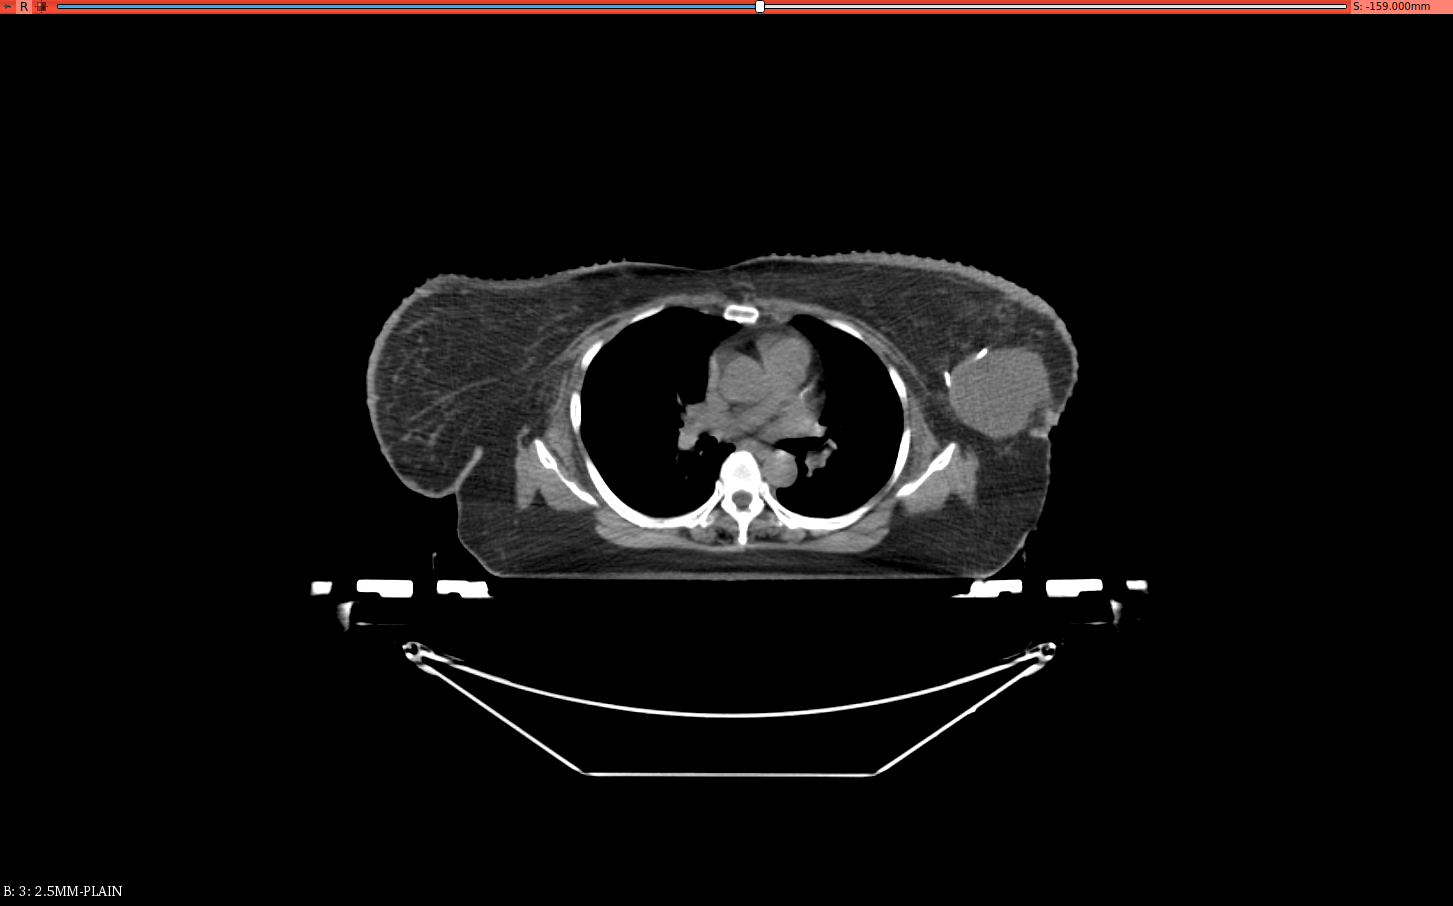
\includegraphics[width=4in]{img2.png}
% \caption{Axial view with the tumor}
% \label{img2}
% \end{figure*}


\begin{figure*}[!b]
\centering
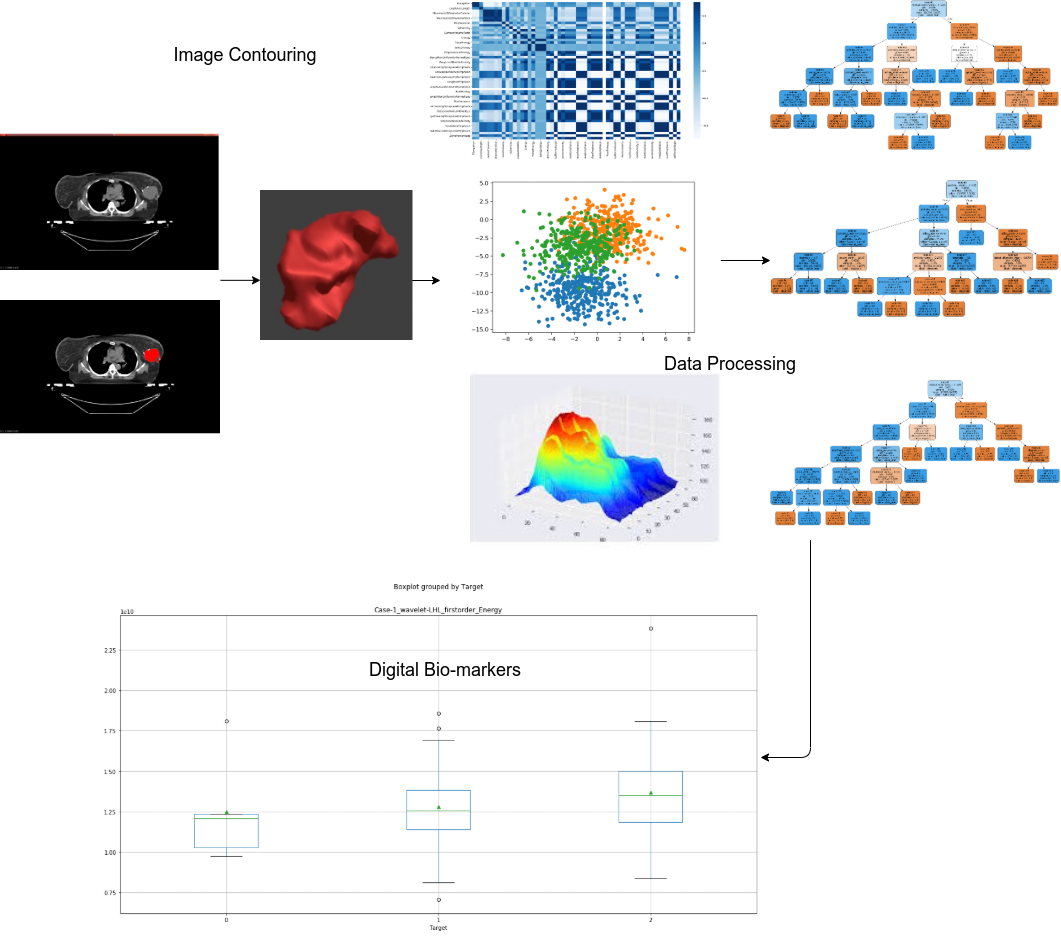
\includegraphics[width=5.4in]{im.png}
\caption{Data-Flow}
\label{img2}
\end{figure*}

\subsection{Convert to a suitable format}

Even though DICOM files are a standard format for medical imaging, NRRD (Nearly Raw Raster Data) files are anonymmized and contain no sensitive patient information in a more compact scheme \cite{12}. NRRD provides a more insightful approach to understanding medical imaging and recognizing inherent patterns in a concised format. The conversion was done with the help of the Plastimatch tool \cite{13}, which is an open source software for image computation. Plastimatch performs rasterization by processing the DICOM image which is described in a polyline vectorized format, and converting it into a series of pixels. The subroutine for rasterization of a DICOM image set with coordinates $x$ and $y$ is shown below.

{\scriptsize
\begin{verbatim}
def rast(x, y, shape):
        nx, ny = draw.polygon(x, y, shape)
        nrrd = np.zeros(shape, dtype=np.bool)
        nrrd[ny, nx] = True 
        return nrrd
\end{verbatim}}

% Once this step is conducted, our image is in a compressed format, rife with information. Information extraction can be conducted through multiple means such as using neural networks, OCR recognition or pattern recognition algorithms. 

\subsection{Obtaining Radiomics Features}

Directly extracting information from images has certain drawbacks. Consider tumor classification using a standard Convolutional Neural Network (CNN). The CNN might be extremely successful in determining the existence of a blob of mass and its exact location. However, diagnosing the precise nature and feature set of the tumor is extremely difficult for a CNN as it views the image as a collection of pixels without any regard for the information embedded in the image.

To tackle this issue, we have utilized radiomics based libraries and algorithms to extract feature sets from the medical images to reveal hidden characteristics. The open-source Python library, PyRadiomics \cite{14}, was used to mine out the required feature set. Before the actual extraction could be performed, a set of filters were applied on the NRRD dataset to provide a comprehensive view of the data. The filters applied are listed in table $\ref{tb2}$. The processing and subsequent image characteristics are discussed in the Supplementary Material.

\begin{table}[!b]
\scriptsize
\centering
\caption{Applied Filters}
\label{tb2}
\begin{tabular}{| l | l | l |}
\hline
\textbf{Filter} & \textbf{Description} & \textbf{Equation}\\
\hline
Wavelet & Selective emphasizing  & -\\
&de-emphasizing of image&\\
\hline
Square & Square the image intensities & x := (cx)\textsuperscript{2}\\
\hline
Square Root & Compute root of image intensities & x := $\sqrt{cx}$\\
\hline
Laplacian of & Applies a Laplacian of Gaussian & $\frac{1}{(\sigma\sqrt{2\pi})\textsuperscript{3}}e\textsuperscript{-\sufr{x\textsuperscript{2}+y\textsuperscript{2}+z\textsuperscript{2}}{2\sigma\textsuperscript{2}}}$\\
Gaussian &fliter for a $\sigma$ value&\\
\hline
Logarithm & Computes the natural logarithm& c$\log(x+1)$\\
& of image intensities &\\
\hline
Exponential & Computes the exponential of & $e\textsuperscript{cx}$\\
&the original image &\\
\hline
Gradient & Computes the gradient of the image & -\\
\hline
\end{tabular}
\end{table}

PyRadiomics extracts radiomics features from the CT scan in a stagewise manner. Initially the images are loaded into the platform by using SimpleITK which supports a gamut of image types along wit basic image processing techniques. In the next step, the filters descibed in $\ref{tb2}$ are applied using SimpleITK \cite{15}, PyWavelets \cite{16}, and Numpy \cite{17}. Finally, statistical and texture classes are used for feature extraction. The features so obtained, are stored in a dictionary format which suitable labels. 

To define a Region of Interest (ROI) and to check the dimensional constraints of the data, a mask file is utilized. The mask file contains the tumor's location demarcated by a radiologist. The features extracted are descibed by the Imaging Biomarker Standardization Initiative (IBSI) \cite{18} and have have been shown in Tables $\ref{tb3}$ and $\ref{tb4}$.
% The mask image corresponding to Figure $\ref{img2}$ is shown in Figure $\ref{img3}$. Note the red mark demarcating the tumor is done by a radiologist as is standard procedure. The features are now extracted from the image set with the help of the mask file. 

% \begin{figure*}[!b]
% \centering
% 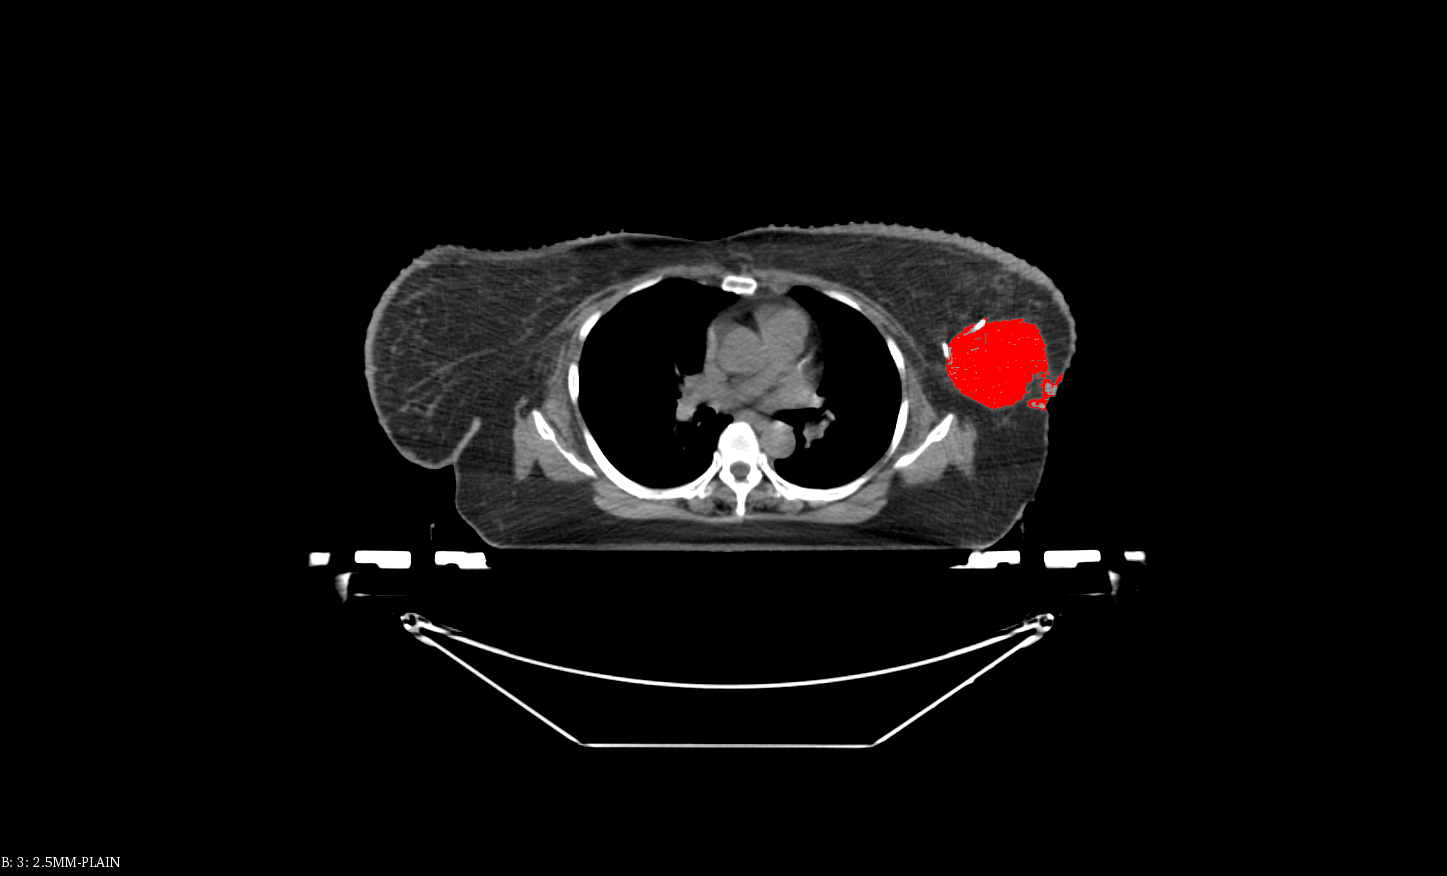
\includegraphics[width=4in]{img3.png}
% \caption{Mask image}
% \label{img3}
% \end{figure*}

\begin{table}[!b]
\scriptsize
\centering
\caption{Features-I}
\label{tb3}
\begin{tabular}{| l | l | l | l | l | l |}
\hline
\textbf{Feature} & \textbf{Feature} & \textbf{Feature} & \textbf{Feature} & \textbf{Feature} & \textbf{Feature}\\
\textbf{Class}&&\textbf{Class}&&\textbf{Class}&\\
\hline
&&&Autocorrelation&&\\
&&&Cluster\_Prominence&&\\
&&&Cluster\_Shade&&\\
&&&Cluster\_Tendency&&High\_Zone\_Emphasis\\
&Max\_2D\_Diameter\_C&&Constrast&&Large\_Area\_Emphasis\\
&Max\_2D\_Diameter\_R&&Correlation&&Large\_Area\_High\_Level\_Emphasis\\
&Max\_2D\_Diameter\_S&&Difference\_Average&&Large\_Area\_Low\_Level\_Emphasis\\
&Max\_3D\_Diameter&&Difference\_Entropy&Grey&Low\_Zone\_Emphasis\\
&Mesh\_Volume&Grey&Difference\_Variance&Level&Zone\_Non\_Uniformity\\
Shape&Minor\_Axis\_Length&Level&Inverse\_Variance&Size&Zone\_Non\_Uniformity\_Normalized\\
&Sphercity&Co-occurance&Joint\_Average&Zone&Small\_Area\_Emphasis\\
&Surface\_Area&Matrix&Joint\_Energy&Matrix&Small\_Area\_High\_Level\_Emphasis\\
&Surface\_Volume&&Joint\_Entropy&&Small\_Area\_Low\_Level\_Emphasis\\
&Voxel\_Volume&&MCC&&Zone\_Entropy\\
&Elongation &&Maximum\_Probability&&Zone\_Percentage\\
&Flatness&&Sum\_Average&&Zone\_Variance\\
&Least\_Axis\_length&&Sum\_Entropy&&Non\_Uniformity\\
&Major\_Axis\_Length&&Sum\_Squares&&Non\_Uniformity\_Normalized\\
&&&Id&&Variance\\
&&&Idm&&\\
&&&Idn&&\\
&&&Idmn&&\\
&&&Imc1&&\\
&&&Imc2&&\\
\hline
&10 Percentile&&&&\\
&90 Percentile&&Normalized\_Uniformity&&\\
&Energy&&Variance&&Dependence\_Non\_Uniformity\_Normalized\\
&Entropy&&High\_Run\_Emphasis&&Dependence\_Variance\\
&Interquartile\_Range&&Long\_Run\_Emphasis&&GL\_Non\_Uniformity\\
&Kurtosis&&Long\_High\_Run\_Emphasis&&GL\_Variance\\
&Maximum&&Long\_Low\_Run\_Emphasis& &High\_Emphasis\\
First &Mean\_Absolute\_Deviation&Grey&Low\_Run\_Emphasis&Gray &Large\_Dependence\_Emphasis\\
Order&Mean&Level&Run\_Entropy&Level&Large\_Dependence\_High\_Emphasis\\
Statistics&Median&Run &Run\_Uniformity&Size&Large\_Dependence\_Low\_Emphasis\\
&Minimum& Length &Normalized\_Uniformity&Zone&Low\_Emphasis\\
&Range&Matrix &Run\_Percentage&Matrix&Small\_Dependence\_Emphasis\\
&Robust\_Mean\_Deviation&&Run\_Variance&&Small\_Dependence\_High\_Emphasis\\
&Robust\_Mean\_Squared&&Short\_Run\_Emphasis&&Small\_Dependence\_Low\_Emphasis\\
&Skewness&&Short\_Run\_High\_Emphasis&&Dependence\_Entropy\\
&Total\_Energy&&Short\_Run\_Low\_Emphasis&&Dependence\_Non\_Uniformity\\
&Uniformity&&Uniformity&&\\
&Variance&&&&\\
\hline
Neighbouring&Busyness&&&&\\
Gray&Coarseness&&&&\\
Tone&Complexity&&&&\\
Difference&Constrast&&&&\\
Matrix&Strength&&&&\\
\hline
\end{tabular}
\end{table}

\begin{table}[!b]
\scriptsize
\centering
\caption{Features-II}
\label{tb4}
\begin{tabular}{| l | l |}
\hline
\textbf{Feature Class} & \textbf{Feature}\\
\hline
&Non\_Uniformity\\
&Non\_Uniformity\_Normalized\\
&Variance\\
&High\_Zone\_Emphasis\\
&Large\_Area\_Emphasis\\
&Large\_Area\_High\_Level\_Emphasis\\
&Large\_Area\_Low\_Level\_Emphasis\\
Grey&Low\_Zone\_Emphasis\\
Level&Zone\_Non\_Uniformity\\
Size&Zone\_Non\_Uniformity\_Normalized\\
Zone&Small\_Area\_Emphasis\\
Matrix&Small\_Area\_High\_Level\_Emphasis\\
&Small\_Area\_Low\_Level\_Emphasis\\
&Zone\_Entropy\\
&Zone\_Percentage\\
&Zone\_Variance\\
\hline
&Dependence\_Entropy\\
&Dependence\_Non\_Uniformity\\
&Dependence\_Non\_Uniformity\_Normalized\\
&Dependence\_Variance\\
&GL\_Non\_Uniformity\\
&GL\_Variance\\
Gray &High\_Emphasis\\
Level &Large\_Dependence\_Emphasis\\
Size&Large\_Dependence\_High\_Emphasis\\
Zone&Large\_Dependence\_Low\_Emphasis\\
Matrix&Low\_Emphasis\\
&Small\_Dependence\_Emphasis\\
&Small\_Dependence\_High\_Emphasis\\
&Small\_Dependence\_Low\_Emphasis\\
\hline
Neighbouring&Busyness\\
Gray&Coarseness\\
Tone&Complexity\\
Difference&Constrast\\
Matrix&Strength\\
\hline
\end{tabular}
\end{table}

Therefore, for each patient, the total number of features obtained are number of filters $\times$ number of features i.e, 17 $\times$ 100 = 1700 features. Once the entire feature set has been collected, the classification task can begin. 

\subsection{Applying Pre-processing Techniques}

From the 1700 features collected, we select a sub-set of top ranking features which contribute significantly to the classification task. The process of preparing the input data for pattern learning by removing redundant characteristics, reducing noises and normalizing, selecting, and extracting features is termed as Data Pre-Processing. We have applied multiple data pre-processing techniques to the feature set, which are listed in Table $\ref{tb5}$.

\begin{table}[!b]
\scriptsize
\centering
\caption{Preprocessing techniques}
\label{tb5}
\begin{tabular}{| l | l |}
\hline
\textbf{Method} & \textbf{Description}\\
\hline
Missing Value Ratio & Removal of data columns where the  \\
&number of missing values $\geq$ threshold\\
\hline
Low Varience Filter & Removal of normalized data columns \\
&where the variance $\leq$ threshold\\
\hline
Highest correlation  & Removal of data columns which are \\
filter&highly correlated leading to redundancy\\
\hline
Principle & Transformation of data to\\
Component Analysis &maximize $\sigma\textsuperscript{2}$ under constraints\\
\hline
Fast Independent & Decomposition of signals to focus  \\
Component Analysis &on mutual independence of data\\
\hline
Factor Analysis & Generating a common feature by \\
&reducing number of common variables \\
\hline
\end{tabular}
\end{table}

Since the number of test subjects for each class is different, a threshold confidence level must be specified during the hypothesis testing phase. A 'P-value' is used to evaluate the hypothesis under observation. A lower p-value corresponds to a higher confidence level in the predictions, thereby accommodating only the information-rich features. The number of features selected after the pre-processing step is directly proportional to the p-value. We created a grid for varying p-values and derived the corresponding number of features for each p-value.   

\subsection{Model-based Predictions}

Once the features have been narrowed down, we initiated the model building process. For any task in hand, we have a wide array of classifiers which accurately predict the nature of the test set. The set of classification algorithms considered are shown in Table $\ref{table:algos}$. In order to determine which algorithm would perform the best for our cohort dataset, we trained all the models on a standard benchmark dataset belonging to the same field i.e, the Winconsin Breast Cancer Diagnostic Dataset. The tabulated results for each algorithm is shown in Table $\ref{table:t1}$.
\begin{table}[!t]
\scriptsize
\caption{Algorithms for traditional and ensembled classification and regression}
\label{table:algos}
\centering
{
\begin{tabular}{| l | l | l | l | }
\hline
\textbf{Index} & \textbf{Algorithm Name} & \textbf{Class} & \textbf{Purpose} \\
\hline
CT1 & Bagged Decision Tree & Traditional & Classification \\
\hline
CT2 & Balanced Bagged Decision Tree & Traditional &  Classification \\
\hline
CT3 & Bagged Random Forest & Traditional &  Classification \\
\hline
CT4 & Balanced Bagged Random Forest & Traditional & Classification \\
\hline
CT5 & Decision Tree & Traditional & Classification \\
\hline
CT6 & K-Nearest Neighbours & Traditional & Classification \\
\hline
CT7 & Neural Network & Traditional & Classification \\
\hline
CE1 & AdaBoost with Decision Tree & Ensemble & Classification (SR)\\
\hline
CE2 & AdaBoost with Decision Tree & Ensemble & Classification (S)\\
\hline
CE3 & AdaBoost with SVM & Ensemble & Classification (SR)\\
\hline
CE4 & AdaBoost with SVM & Ensemble & Classification (S)\\
\hline
CE5 & RUSBoost with Decision Tree & Ensemble & Classification (SR)\\
\hline
CE6 & RUSBoost with Decision Tree & Ensemble & Classification (S)\\
\hline
CE7 & RUSBoost with Random Forest & Ensemble & Classification (SR)\\
\hline
CE8 & RUSBoost with Random Forest & Ensemble & Classification (S)\\
\hline
CE9 & RUSBoost with SVM & Ensemble & Classification (SR)\\
\hline
CE10 & RUSBoost with SVM & Ensemble & Classification (S)\\
\hline
\end{tabular}
}
\end{table}

\begin{table*}[!t]
\scriptsize
\caption{Performance Analysis}
\label{table:t1}
\centering
\scalebox{0.95}
{
\begin{tabular}{| l | l | l | l | l | l | l | l | l | l | l | l | l | l | l | l | l | l | l | l |}
\hline
\textbf{Model} & {CT1} & {CT2} & {CT3} & {CT4} & {CT5} & {CT6} & {CT7} & {CE1} & {CE2}\\
\hline
\textbf{Accuracy Reading}& 0.9917 & 0.9870 & 0.9959 & 0.9959 & 0.9651 & 0.9949 & 1.0000 & 0.8713 & 0.9709\\
\hline
\textbf{Time Taken}& 44.2017 & 44.2017 & 27.9943 & 27.9943 & 15.5171 & 18.6339 & 26.5288 & 127.2628 & 127.2628\\
\hline
&&&&&&&&&\\
\hline
\textbf{Model} & {CE3} & {CE4} & {CE5} & {CE6} & {CE7} & {CE8} & {CE9} & {CE10} & \textbf{SFORCE} \\
\hline
\textbf{Accuracy Reading}& 1.0000 & 1.0000 & 0.9870 & 0.9896 & 1.0000 & 0.9977 & 0.9920 & 0.9977 & \textbf{0.9974} \\
\hline
\textbf{Time Taken}& 54.6694 & 54.6694 & 156.7184 & 156.7184 & 24.2733 & 24.2733 & 27.1538 & 27.1538 & \textbf{570.5684} \\
\hline
\end{tabular}
}
\end{table*}
% 
% \begin{table*}[!t]
% \caption{Performance Analysis II}
% \label{table:t2}
% \centering
% \scalebox{0.7}
% {
% \begin{tabular}{| l | l | l | l | l | l | l | l | l | l | l | l | l | l | l | l | l | l | l | l |}
% \hline
% {Model} & {CE3} & {CE4} & {CE5} & {CE6} & {CE7} & {CE8} & {CE9} & {CE10} & \textbf{SFORCE (SR)} & \textbf{SFORCE (SR) with K-Fold cross validation} \\
% \hline
% Accuracy Reading  & 1.0000 & 1.0000 & 0.9870 & 0.9896 & 1.0000 & 0.9977 & 0.9920 & 0.9977 & \textbf{0.9958} & \textbf{0.9974} \\
% \hline
% Time Taken & 54.6694 & 54.6694 & 156.7184 & 156.7184 & 24.2733 & 24.2733 & 27.1538 & 27.1538 & \textbf{220.5434} & \textbf{570.5684} \\
% \hline
% \end{tabular}
% }
% \end{table*}

As determined, SFORCE (post validation) provides promising results without overfitting and hence is used to classify test subjects into the target classes. SFORCE establishes a symbiotic relation between a predictive model (Random Forest) and an Ensemble model (AdaBoost). Both these models work on the presented data simultaneously, aiding each other in the prediction process. Random Forests provides a strong learning system with the occasional pitfall of overfitting. The algorithms are discussed in-depth in the supplementary material. 

% The data is classified based the features which contrast the classes with the highest information content. The process of data classification using Random Forest is shown in Algorithm $\ref{alg:rf}$. AdaBoost solves the problem of overfitting by presenting the system with the misclassified data and forcing it to improve the overall performance. The two flavours of AdaBoost i.e, SAMME and SAMME.R have been descibed in Algorithms $\ref{alg:samme}$ and $\ref{alg:sammer}$. SFORCE combines the strength of Random Forests and takes care of the  drawbacks by using a Boosting algorithm to make the search process more concentrated as shown in Algorithm $\ref{alg:sforce}$. 

To obtain digital bio-markers, we conducted two case studies on the avaiable cohort dataset. The first study involved classifying test subjects as TN or non TN subjects. In the second study, the Luminal-B dataset was set aside as the test dataset due to the close resemblance of its characteristics with those of Luminal A. We trained the model to place the test subjects into the Luminal-A class, resulting in an accuracy of 72.7\%. The results for different p-values are described in Tables $\ref{tb6}$ and $\ref{tb7}$. Based on these results, we obtained the box-plots for the selected features which act as bio-markers for future reference.


\begin{table}[!b]
\scriptsize
\centering
\caption{TN vs Non-TN}
\label{tb6}
\begin{tabular}{| c | c | c | c |}
\hline
\textbf{P-Value} & \textbf{Number of} & \textbf{Accuracy} & \textbf{Accuracy}\\
&Features&(SAMME)&(SAMME.R)\\
\hline
1&20&81.25&90.39\\
\hline
0.5&16&90.39&93.25\\
\hline
0.1&6&75&81.25\\
\hline
\end{tabular}
\end{table}

\begin{table}[!b]
\scriptsize
\centering
\caption{HER vs Luminal-A vs TN}
\label{tb7}
\begin{tabular}{| c | c | c | c |}
\hline
\textbf{P-Value} & \textbf{Number of} & \textbf{Accuracy} & \textbf{Accuracy}\\
&Features&(SAMME)&(SAMME.R)\\
\hline
1E-5&16&72&63.63\\
\hline
1E-6&15&70&72.7\\
\hline
1E-7&13&72.7&70\\
\hline
\end{tabular}
\end{table}

% \begin{algorithm}
% \begin{algorithmic}[1]
% \STATE Start
% \end{algorithmic}
% \end{algorithm}

\subsection{Role of source funding}

The funders had no role in study design, data interpretation, writing of the manuscript, and decision to submit. All the authors had full access to all the data used in the study and had final responsibility for the decision to submit for publication.

\section{Results and Conclusion}

From the data-driven pipeline, we obtained the quantifiable digital biomarkers in the form of box and whisker plots. These plots provide a convenient method of displaying the data distribution and provide insight to the oncological expert during prognosis of future test subjects. Sample box plots are displayed in Figures $\ref{b1}$ to $\ref{b4}$. The entire list of digital biomarkers along with their corresponding box plots are included in the supplementary material. Note that the number of digital biomarkers correspond to the number of the box plots, which in turn corresponds to number of mappings between features and filters selected. 

The pipeline developed for this study consists of multidisciplinary stages with involvement of both Radiomics and modern statistics \cite{22}. While Radiomics provides a real-world application based avenue, statistical tools were used to narrow down our biomarker search process. The aim of condensing the number of features is to preserve the features with the highest level information embedded in them. 

However it must also be duely noted that this pipeline is quite delicate when it comes to producing results as the errors encountered in each step are rippled onto the next stages. Furthermore an increased sample dataset size could help further fine tune the model. Additional Deep Learning frameworks can also be introduced to provide competition to the incumbent design model.  
% 
% \begin{figure}[t]
% \begin{subfigure}{}
%   \centering
%   % include first image
%   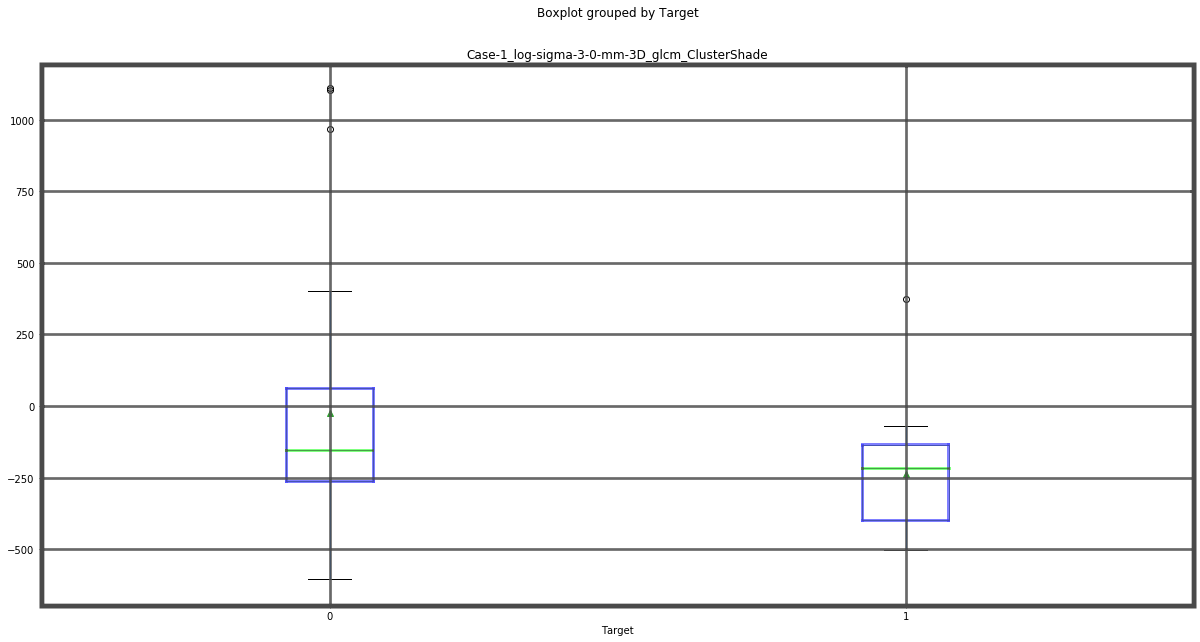
\includegraphics[width=.8\linewidth]{bg1.png}  
% %   \caption{Put your sub-caption here}
%   \label{fig:sub-first}
% \end{subfigure}
% \begin{subfigure}{}
%   \centering
%   % include second image
%   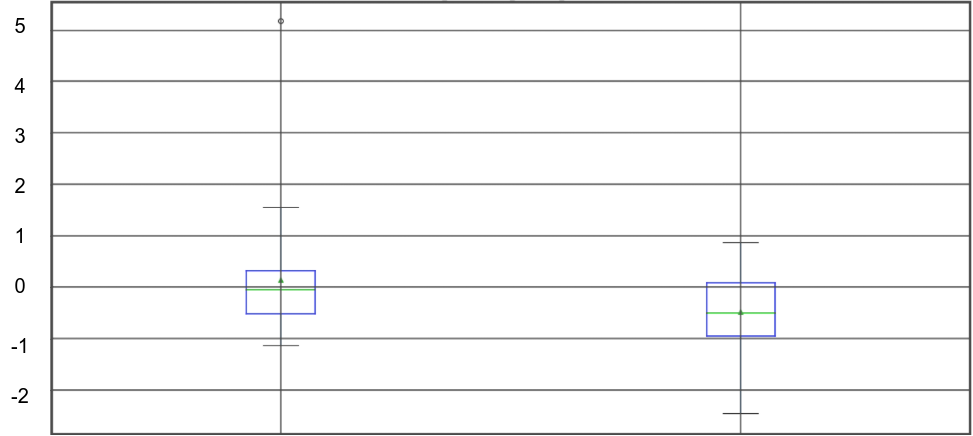
\includegraphics[width=.8\linewidth]{bg2.png}  
% %   \caption{Put your sub-caption here}
%   \label{fig:sub-second}
% \end{subfigure}
% \begin{subfigure}{}
%   \centering
%   % include first image
%   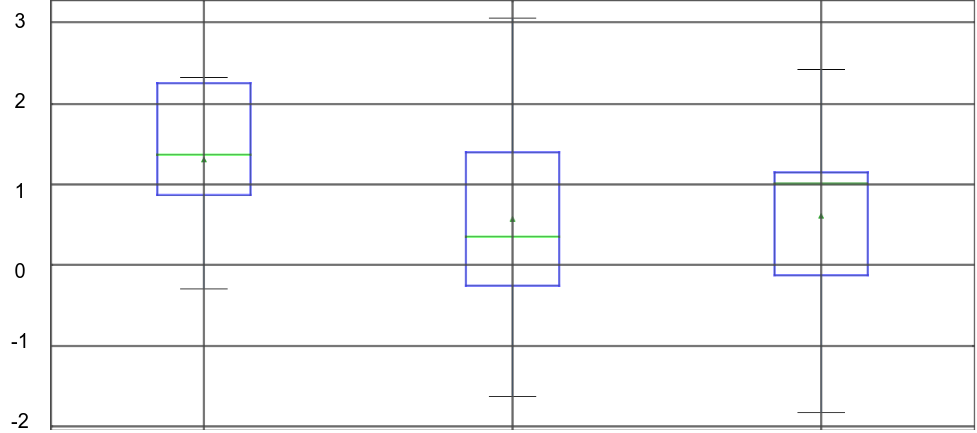
\includegraphics[width=.8\linewidth]{tg1.png}  
% %   \caption{Put your sub-caption here}
%   \label{fig:sub-first}
% \end{subfigure}
% \begin{subfigure}{}
%   \centering
%   % include second image
%   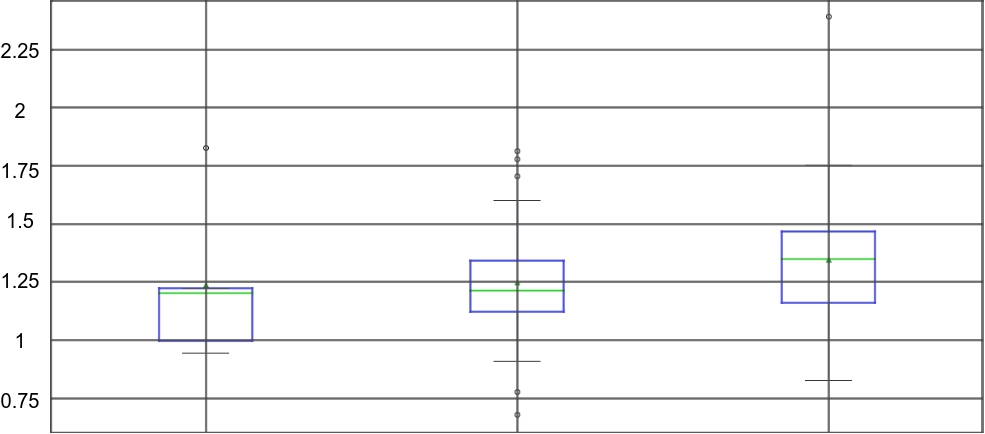
\includegraphics[width=.8\linewidth]{tg2.png}  
% %   \caption{Put your sub-caption here}
%   \label{fig:sub-second}
% \end{subfigure}
% \caption{Sample Box Plots}
% \end{figure}
% 

% \begin{figure}
% \begin{subfigure}{}
%   \centering
%   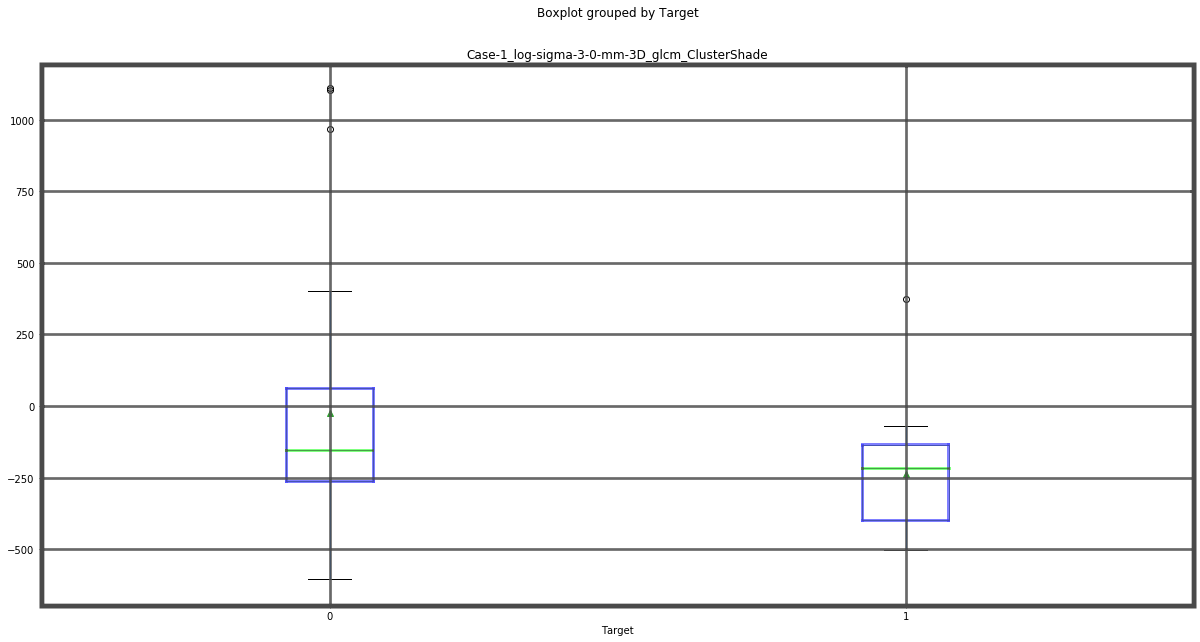
\includegraphics[width=8cm]{bg1.png}
%   \caption{}
%   \label{fig:sfig1}
% \end{subfigure}%
% \begin{subfigure}{}
%   \centering
%   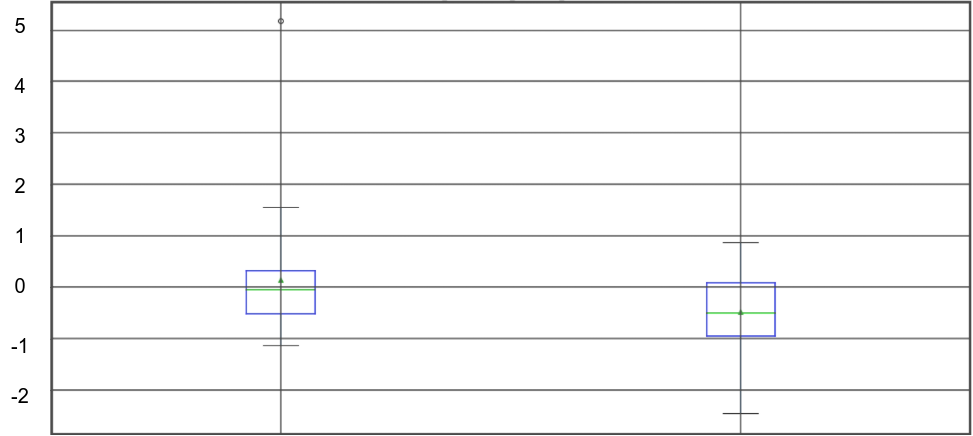
\includegraphics[width=8cm]{bg2.png}
%   \caption{}
%   \label{fig:sfig2}
% \end{subfigure}
% \begin{subfigure}{}
%   \centering
%   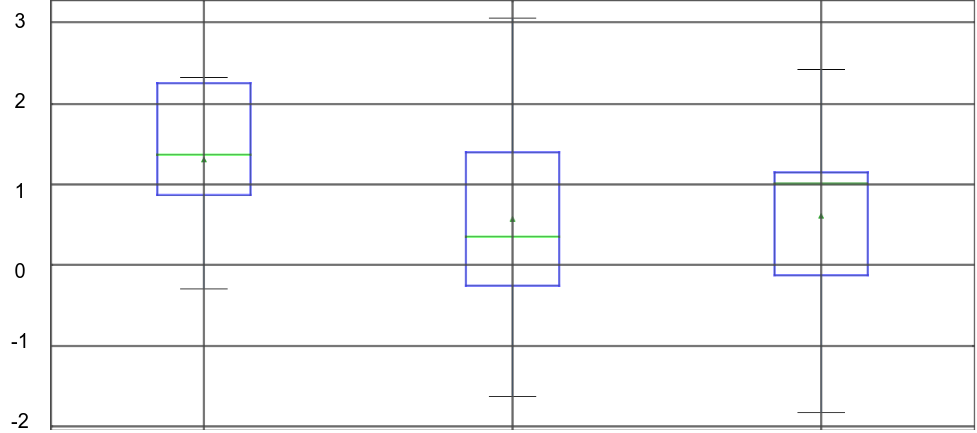
\includegraphics[width=8cm]{tg1.png}
%   \caption{}
%   \label{fig:sfig3}
% \end{subfigure}%
% \begin{subfigure}{}
%   \centering
%   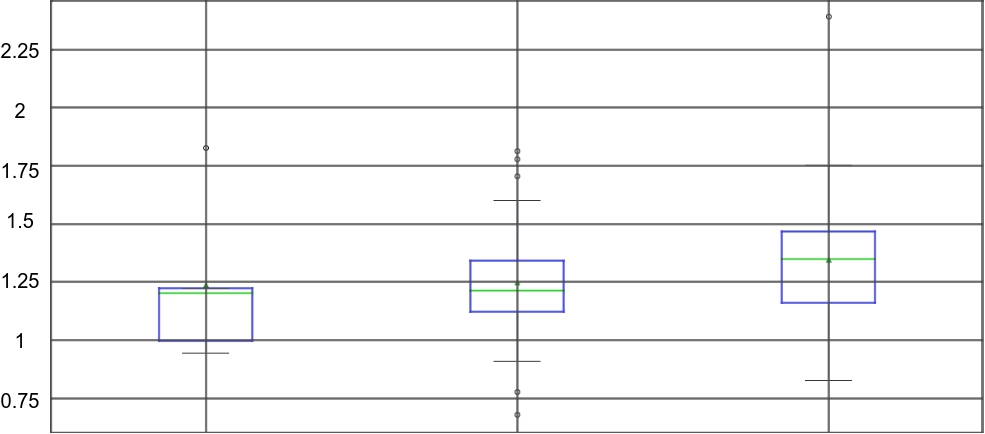
\includegraphics[width=8cm]{tg2.png}
%   \caption{}
%   \label{fig:sfig4}
% \end{subfigure}
% % \caption{plots of....}
% % \label{fig:fig}
% \end{figure}



\begin{figure}
    \centering
    \begin{minipage}{0.45\textwidth}
        \centering
        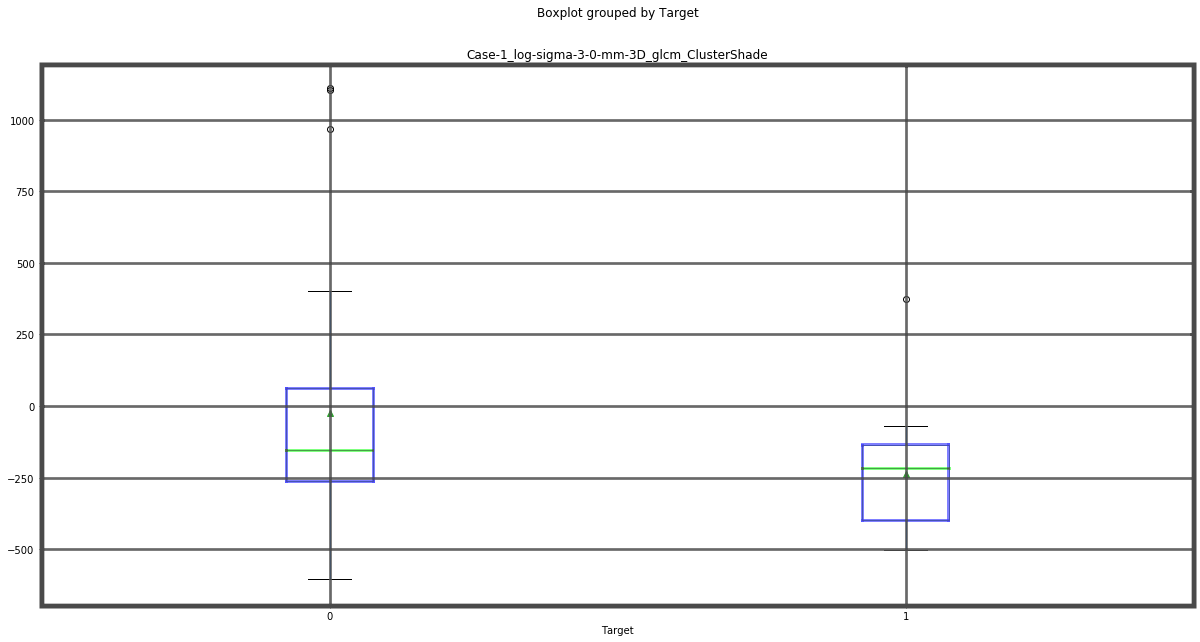
\includegraphics[width=0.9\textwidth]{bg1.png} % first figure itself
        \caption{Sample Box and wiskhers plot for TN (left) vs Non-TN (right)}
        \label{b1}
    \end{minipage}\hfill
    \begin{minipage}{0.45\textwidth}
        \centering
        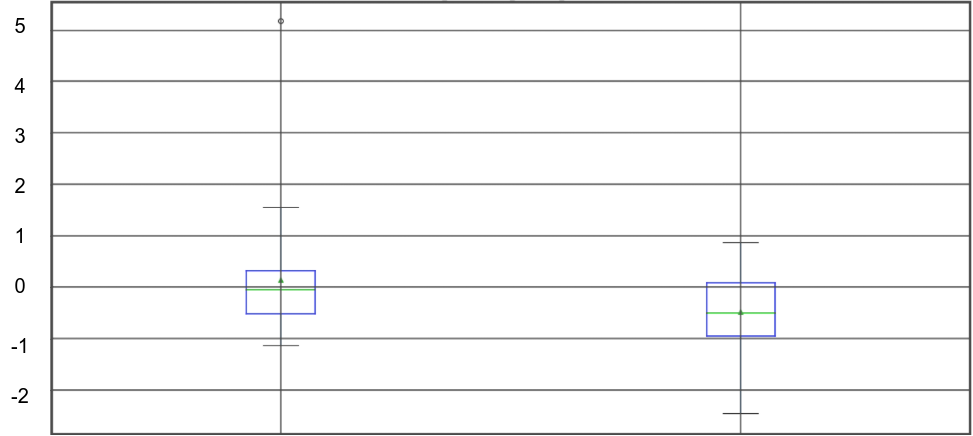
\includegraphics[width=0.9\textwidth]{bg2.png} % second figure itself
        \caption{Sample Box and wiskhers plot for TN (left) vs Non-TN (right)}
        \label{b2}
    \end{minipage}
    \begin{minipage}{0.45\textwidth}
        \centering
        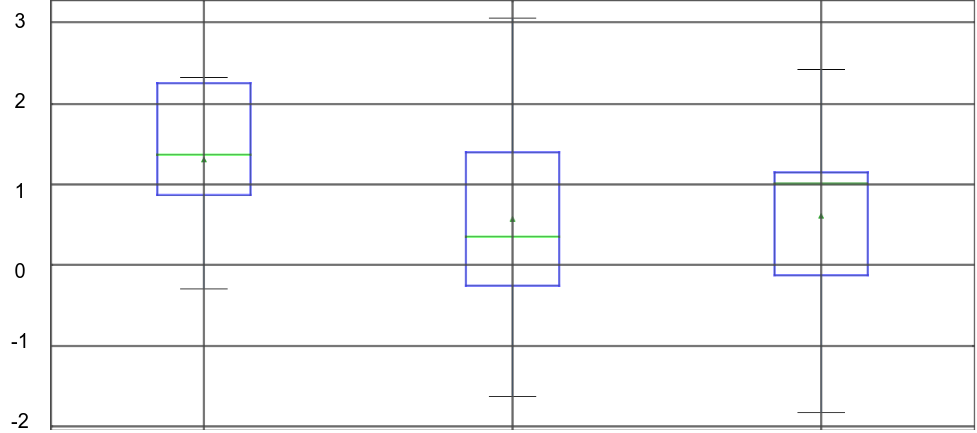
\includegraphics[width=0.9\textwidth]{tg1.png} % first figure itself
        \caption{Sample Box and wiskhers plot for HER (left) vs Luminal-A (center) vs TN (right)}
        \label{b3}
    \end{minipage}\hfill
    \begin{minipage}{0.45\textwidth}
        \centering
        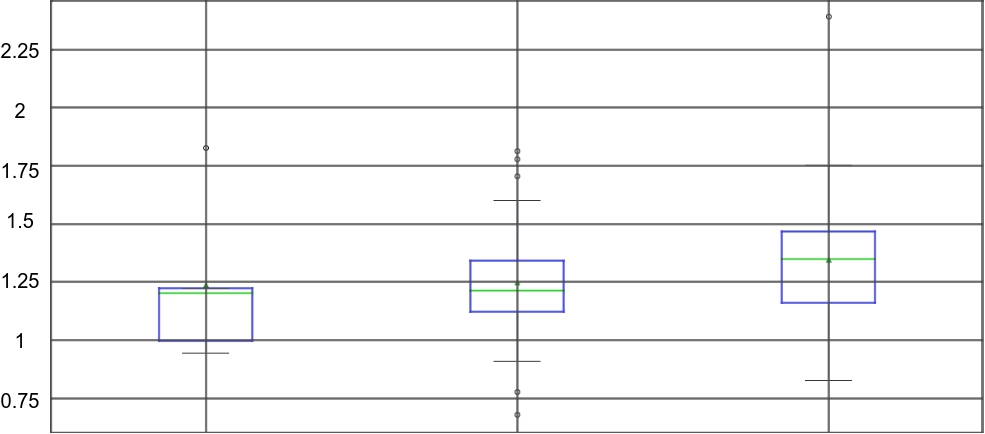
\includegraphics[width=0.9\textwidth]{tg2.png} % second figure itself
        \caption{Sample Box and wiskhers plot for HER (left) vs Luminal-A (center) vs TN (right)}
        \label{b4}
    \end{minipage}
\end{figure}


% 
% \begin{figure}
% \centering
% 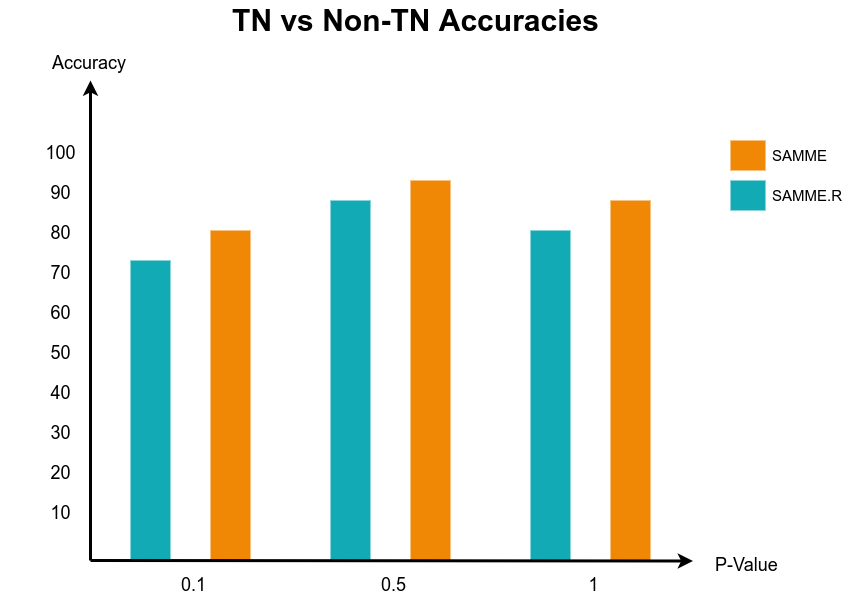
\includegraphics[width=3in]{acc1.png}
% \caption{TN vs Non-TN Classification Accuracies}
% \label{img5}
% \end{figure}
% 
% \begin{figure}
% \centering
% 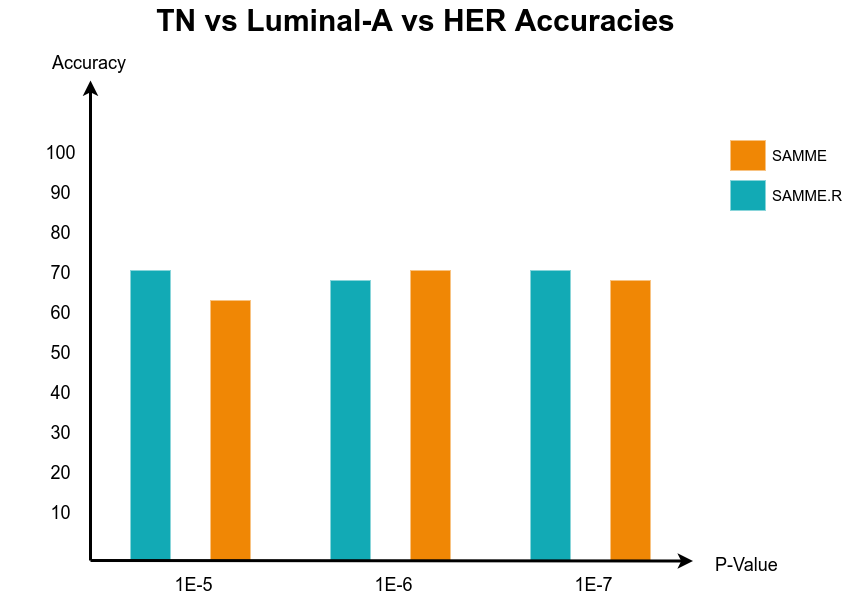
\includegraphics[width=3in]{acc2.png}
% \caption{TN vs Luminal-A vs HER Classification Accuracies}
% \label{img6}
% \end{figure}



\begin{figure}
    \centering
    \begin{minipage}{0.45\textwidth}
        \centering
        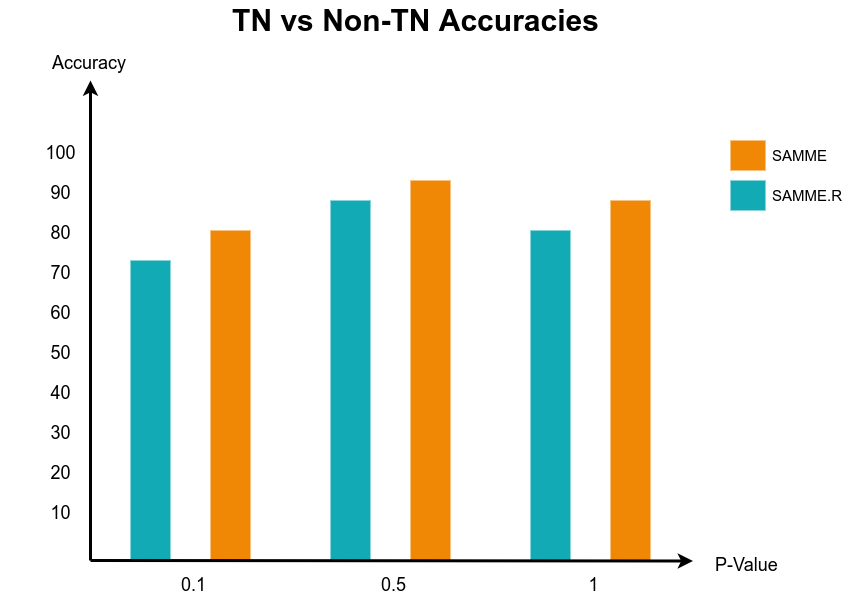
\includegraphics[width=0.9\textwidth]{acc1.png} % first figure itself
    \end{minipage}\hfill
    \begin{minipage}{0.45\textwidth}
        \centering
        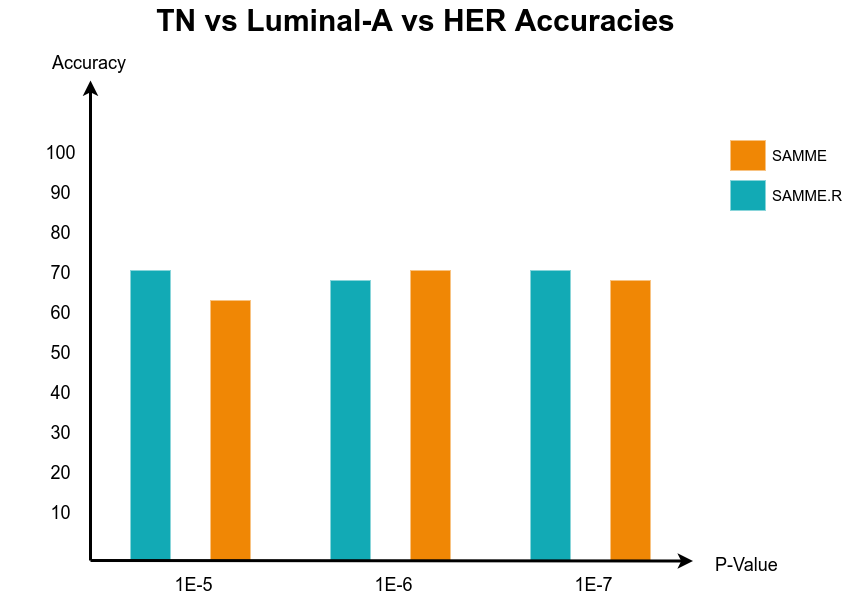
\includegraphics[width=0.9\textwidth]{acc2.png} % second figure itself
    \end{minipage}
\end{figure}


\subsection{Contributors}

% \author[label1]{Santhi Natarajan, Anand Ravishankar, Bharathi Malakreddy A}
% \author[label2]{G.Lohith, Kritika Sekar, Shivakumar Swamy, Kumar Kallur, Basavalinga Ajai Kumar, Mahesh Bandimegal, Krithika Murugan}

The Radiogenomics Research Group of BMS Institute of Technology and Management developed the Image Processing Pipeline with Machine Learning algorithmic steps, and has also executed them on computing platforms, producing the results discussed in the paper. The oncological research team within the HCG group served as the medical partner and provided the data for Indian breast cancer cohort with multiple molecular subtypes, as well as other ethical clearances for conducting this cross-reference study on the cohort. All authors have contributed to the formulation of the reseaarch statement, methodology, installation, execution and verfication of the findings and mapping of results to inferences. All authors contributed to the writing of the final version of the Article.

\subsection{Declaration of interests}
We declare no competing interests.

\subsection{Data Sharing}



\subsection{Acknowledgment}

The authors would like to thank the Vision Group on Science and Technology, Government of Karnataka, India, for funding this project under the Centre for Design and Research on Healthcare Applications using AI. The authors also would like to thank the HCG management for support provided to obtain the ethical clearances for this study.

%% The Appendices part is started with the command \appendix;
%% appendix sections are then done as normal sections
%% \appendix

%% \section{}
%% \label{}

%% References
%%
%% Following citation commands can be used in the body text:
%% Usage of \cite is as follows:
%%   \cite{key}          ==>>  [#]
%%   \cite[chap. 2]{key} ==>>  [#, chap. 2]
%%   \citet{key}         ==>>  Author [#]

%% References with bibTeX database:

\bibliographystyle{model1-num-names}
\bibliography{sample.bib}



%% Authors are advised to submit their bibtex database files. They are
%% requested to list a bibtex style file in the manuscript if they do
%% not want to use model1-num-names.bst.

%% References without bibTeX database:

\begin{thebibliography}{00}

%% \bibitem must have the following form:
%%   \bibitem{key}...
%%

\bibitem{1} Heather D. Couture1 Lindsay A. Williams, Joseph Geradts Sarah J. Nyante Ebonee N. Butler J. S. Marron, Charles M., Perou Melissa A. Troester and Marc Niethammer. Image analysis with deep learning to predict breast cancer grade, ER status, histologic subtype, and intrinsic subtype. Nature Partner Journals (2018)
\bibitem{2} Lohmann, P., Bousabarah, K., Hoevels, M. et al. Radiomics in radiation oncology—basics, methods, and limitations. Strahlenther Onkol 196, 848–855 (2020). https://doi.org/10.1007/s00066-020-01663-3. 
\bibitem{d} Robertson S, Azizpour H, Smith K, Hartman J. Digital image analysis in breast pathology-from image processing techniques to artificial intelligence. Transl Res. 2018 Apr;194:19-35. doi: 10.1016/j.trsl.2017.10.010. Epub 2017 Nov 7. PMID: 29175265.
\bibitem{e} Jaber MI, Song B, Taylor C, Vaske CJ, Benz SC, Rabizadeh S, Soon-Shiong P, Szeto CW. A deep learning image-based intrinsic molecular subtype classifier of breast tumors reveals tumor heterogeneity that may affect survival. Breast Cancer Res. 2020 Jan 28;22(1):12. doi: 10.1186/s13058-020-1248-3
\bibitem{3} Carelli S, Giallongo T, Rey F, Barzaghini B, Zandrini T, Pulcinelli A, Nardomarino R, Cerullo G, Osellame R, Cereda C, Zuccotti GV, Raimondi MT. Neural precursors cells expanded in a 3D micro-engineered niche present enhanced therapeutic efficacy in vivo. Nanotheranostics 2021; 5(1):8-26. doi:10.7150/ntno.50633. Available from https://www.ntno.org/v05p0008.htm
\bibitem{4} Blows, Fiona \& Driver, Kristy \& Schmidt, Marjanka \& Broeks, Annegien \& Leeuwen, Flora \& Wesseling, Jelle \& Cheang, Maggie \& Gelmon, Karen \& Nielsen, Torsten \& Blomqvist, Carl \& Heikkilä, Päivi \& Heikkinen, Tuomas \& Nevanlinna, Heli \& Akslen, Lars \& Bégin, Louis \& Foulkes, William \& Couch, Fergus \& Wang, Xianshu \& Cafourek, Vicky \& Huntsman, David. (2010). Subtyping of Breast Cancer by Immunohistochemistry to Investigate a Relationship between Subtype and Short and Long Term Survival: A Collaborative Analysis of Data for 10,159 Cases from 12 Studies. PLoS medicine. 7. e1000279. 10.1371/journal.pmed.1000279.
\bibitem{5} Liu YX, Wang KR, Xing H, Zhai XJ, Wang LP, Wang W. Attempt towards a novel classification of triple-negative breast cancer using immunohistochemical markers. Oncol Lett. 2016 Aug;12(2):1240-1256. doi: 10.3892/ol.2016.4778. Epub 2016 Jun 23. PMID: 27446423; PMCID: PMC4950427.
\bibitem{6} Arnaud Marcoux, Ninon Burgos, Anne Bertrand, Marc Teichmann, Alexandre Routier, et al.. An Au-
tomated Pipeline for the Analysis of PET Data on the Cortical Surface. Frontiers in Neuroinformatics, Frontiers, 2018, 12, ff10.3389/fninf.2018.00094ff. ffhal-01950933ff
\bibitem{7} Xie T, Wang Z, Zhao Q, et al. Machine Learning-Based Analysis of MR Multiparametric Radiomics for the Subtype Classification of Breast Cancer. Front Oncol. 2019;9:505. Published 2019 Jun 14. doi:10.3389/fonc.2019.00505
\bibitem{a} Shaikh FA, Kolowitz BJ, Awan O, Aerts HJ, von Reden A, Halabi S, Mohiuddin SA, Malik S, Shrestha RB, Deible C. Technical Challenges in the Clinical Application of Radiomics. JCO Clin Cancer Inform. 2017 Nov;1:1-8. doi: 10.1200/CCI.17.00004. PMID: 30657374.
\bibitem{8} van Timmeren JE, Cester D, Tanadini-Lang S, Alkadhi H, Baessler B. Radiomics in medical imaging-"how-to" guide and critical reflection. Insights Imaging. 2020;11(1):91. Published 2020 Aug 12. doi:10.1186/s13244-020-00887-2
\bibitem{9} Gillies RJ, Kinahan PE, Hricak H. Radiomics: Images Are More than Pictures, They Are Data. Radiology. 2016 Feb;278(2):563-77. doi: 10.1148/radiol.2015151169. Epub 2015 Nov 18. PMID: 26579733; PMCID: PMC4734157.
\bibitem{10} Panayides, Andreas \& Pattichis, Marios \& Leandrou, Stephanos \& Pitris, Costas \& Constantinidou, Anastasia \& Pattichis, C.. (2019). Radiogenomics for Precision Medicine With A Big Data Analytics Perspective. IEEE Journal of Biomedical and Health Informatics. 23. 2063-2079. 10.1109/JBHI.2018.2879381. 
\bibitem{11} Tsougos, Ioannis \& Vamvakas, Alexandros \& Kappas, Constantin \& Fezoulidis, Ioannis \& Vassiou, Katerina. (2018). Application of Radiomics and Decision Support Systems for Breast MR Differential Diagnosis. Computational and Mathematical Methods in Medicine. 2018. 1-8. 10.1155/2018/7417126.
\bibitem{b} Sengal AT, Haj-Mukhtar NS, Elhaj AM, Bedri S, Kantelhardt EJ, Mohamedani AA. Immunohistochemistry defined subtypes of breast cancer in 678 Sudanese and Eritrean women; hospitals based case series. BMC Cancer. 2017 Dec 1;17(1):804. doi: 10.1186/s12885-017-3805-4. PMID: 29191181; PMCID: PMC5710067.
\bibitem{c} Tang P, Tse GM. Immunohistochemical Surrogates for Molecular Classification of Breast Carcinoma: A 2015 Update. Arch Pathol Lab Med. 2016 Aug;140(8):806-14. doi: 10.5858/arpa.2015-0133-RA. PMID: 27472239.
\bibitem{12} Larobina M, Murino L. Medical image file formats. J Digit Imaging. 2014;27(2):200-206. doi:10.1007/s10278-013-9657-9
\bibitem{13} Sharp, G. \& LI, R. \& Wolfgang, John \& Chen, G. \& Peroni, Marta \& Spadea, Maria \& Mori, Shinichiro \& Zhang, J. \& Shackleford, J. \& Kandasamy, Nagarajan. (2010). PLASTIMATCH– AN OPEN SOURCE SOFTWARE SUITE FOR RADIOTHERAPY IMAGE PROCESSING.
\bibitem{14}  van Griethuysen, J. J. M., Fedorov, A., Parmar, C., Hosny, A., Aucoin, N., Narayan, V., Beets-Tan, R. G. H., Fillon-Robin, J. C., Pieper, S., Aerts, H. J. W. L. (2017). Computational Radiomics System to Decode the Radiographic Phenotype. Cancer Research, 77(21), e104–e107. `https://doi.org/10.1158/0008-5472.CAN-17-0339 <https://doi.org/10.1158/0008-5472.CAN-17-0339>
\bibitem{15} R. Beare, B. C. Lowekamp, Z. Yaniv, “Image Segmentation, Registration and Characterization in R with SimpleITK”, J Stat Softw, 86(8), doi: 10.18637/jss.v086.i08, 2018.
\bibitem{16} Gregory R. Lee, Ralf Gommers, Filip Wasilewski, Kai Wohlfahrt, Aaron O'Leary (2019). PyWavelets: A Python package for wavelet analysis.
\bibitem{17} Harris, C.R., Millman, K.J., van der Walt, S.J. et al. Array programming with NumPy. Nature 585, 357–362 (2020).
\bibitem{18} Zwanenburg A, Vallières M, Abdalah MA, Aerts HJWL, Andrearczyk V, Apte A, Ashrafinia S, Bakas S, Beukinga RJ, Boellaard R, Bogowicz M, Boldrini L, Buvat I, Cook GJR, Davatzikos C, Depeursinge A, Desseroit MC, Dinapoli N, Dinh CV, Echegaray S, El Naqa I, Fedorov AY, Gatta R, Gillies RJ, Goh V, Götz M, Guckenberger M, Ha SM, Hatt M, Isensee F, Lambin P, Leger S, Leijenaar RTH, Lenkowicz J, Lippert F, Losnegård A, Maier-Hein KH, Morin O, Müller H, Napel S, Nioche C, Orlhac F, Pati S, Pfaehler EAG, Rahmim A, Rao AUK, Scherer J, Siddique MM, Sijtsema NM, Socarras Fernandez J, Spezi E, Steenbakkers RJHM, Tanadini-Lang S, Thorwarth D, Troost EGC, Upadhaya T, Valentini V, van Dijk LV, van Griethuysen J, van Velden FHP, Whybra P, Richter C, Löck S. The Image Biomarker Standardization Initiative: Standardized Quantitative Radiomics for High-Throughput Image-based Phenotyping. Radiology. 2020 May;295(2):328-338. doi: 10.1148/radiol.2020191145. Epub 2020 Mar 10. PMID: 32154773; PMCID: PMC7193906.
\bibitem{22} Giraud P, Gasnier A, et al. Radiomics and Machine Learning for Radiotherapy in Head and Neck Cancers. Front Oncol. 2019;9:174. Published 2019 Mar 27. doi:10.3389/fonc.2019.00174
\end{thebibliography}


\end{document}

%%
%% End of file `elsarticle-template-1-num.tex'.
